% ********** Rozdział 2 **********
\chapter{Opis struktury projektu}
\section{Podstawowe informacje techniczne}
Aplikacja została napisana w języku C\# i uruchamiana jest w konsoli.

\section{Minimalne wymagania sprzętowe}
\begin{itemize}
    \item Procesor minimum 2 GHz.
    \item 2 GB pamięci RAM.
    \item System operacyjny Windows/Linux.
    \item Zainstalowane środowisko .NET.
\end{itemize}

\section{Hierarchia klas}

System składa się z hierarchii klas, które reprezentują różne typy pojazdów oraz logikę zarządzania parkingiem. 
Podstawową klasą jest \textbf{Pojazd}, która jest klasą abstrakcyjną i stanowi bazę dla klas: \textbf{Motocykl}, \textbf{Samochod} oraz \textbf{Autobus}. 
Klasa \textbf{Parking} odpowiada za zarządzanie pojazdami i przechowywanie ich stanu. 
Program steruje aplikacją i zapewnia interakcję z użytkownikiem.

\section{Diagram klas}

Poniżej przedstawiono diagram klas UML obrazujący relacje między klasami w systemie:

\begin{itemize}
    \item \textbf{Program} – klasa główna, odpowiedzialna za uruchomienie aplikacji i zarządzanie logiką programu.
    \item \textbf{Parking} – klasa zarządzająca stanem parkingu, przechowująca informacje o zajętych miejscach oraz umożliwiająca dodawanie i usuwanie pojazdów.
    \item \textbf{Pojazd} – klasa bazowa dla różnych typów pojazdów, przechowuje informacje o numerze rejestracyjnym, typie pojazdu oraz zajmowanych miejscach parkingowych.
    \begin{itemize}
        \item \textbf{Motocykl} – klasa dziedzicząca po klasie Pojazd, reprezentująca motocykl na parkingu.
        \item \textbf{Samochód} – klasa dziedzicząca po klasie Pojazd, reprezentująca standardowy samochód osobowy.
        \item \textbf{Autobus} – klasa dziedzicząca po klasie Pojazd, zajmująca większą liczbę miejsc na parkingu.
    \end{itemize}
\end{itemize}

\subsection{Schemat klas}
Powyżej przedstawiony jest diagram klas obrazujący zależności między poszczególnymi elementami systemu.

\begin{figure}[]
    \centering
    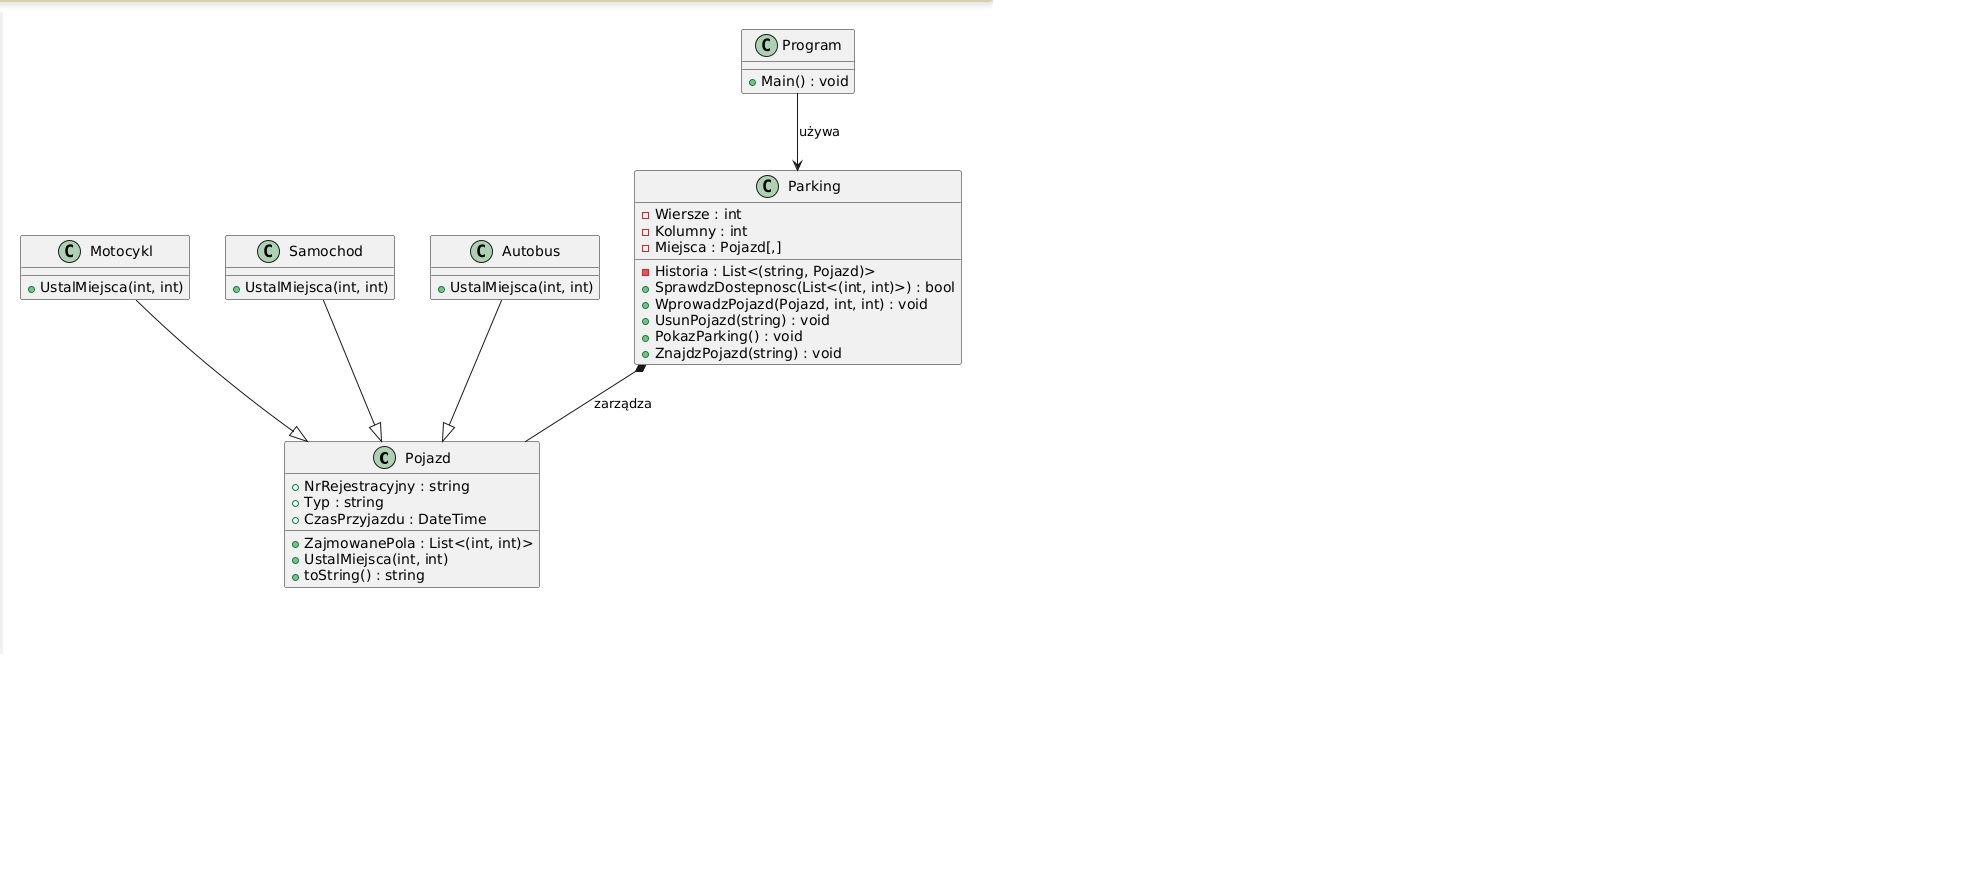
\includegraphics[width=\textwidth]{diagram_klas2.jpg}
    \caption{Diagram klas systemu parkingowego}
    \label{fig:diagram_klas}
\end{figure}






% ********** Koniec rozdziału **********
